\documentclass[notitlepage]{article}
\usepackage{fancyhdr}
\usepackage{amsmath}
\usepackage{listings}
\usepackage[top=0.5in, left=0.85in, right=0.85in]{geometry}
\usepackage{bera}
\usepackage[shortlabels]{enumitem}
\usepackage{graphicx}



\newtheorem{theorem}{Theorem}
\newtheorem{lemma}{Lemma}
\newtheorem{definition}{Definition}
\newtheorem{property}{Property}

\date{}
\title{{\large CSE 515: Statistical Methods in Computer Science}\\ Homework Assignment 2}
\author{Chenglong Wang}

\begin{document}

\maketitle

\section{Kalman Filters}
\begin{enumerate} 
\item We can calculate $P(\mathbf{X}_1)$ as follows:
\begin{align*}
P(\mathbf{X}_1) = & \int_{x}\sum_{i}^{k}P(\mathbf{X}_1|S_0=i, X_0=x)P(S_0=i)P(X_0=x)dx\\
								= & \sum_{i}^{k}P(S_0=i)\int_{x}P(\mathbf{X}_1|S_0=i, X_0=x)P(X_0=x)dx
\end{align*}
Note that in the last step formula, $P(\mathbf{X}_1|S_0=i, X_0=x)$ and $P(X_0=x)$ are both Gaussians, and their product is also Gaussian. Secondly, the integral of a Gaussian remains a Gaussian, so that $P(\mathbf{X}_1)$ is a mixure of Gaussian with the proceeding  sum over all switches.

\item First, we calculate $P(\mathbf{X}_{t+1} | e_{1:t})$:
\begin{align*}
P(\mathbf{X}_{t+1} | e_{1:t}) = & \int_{x}\sum_{i}P(\mathbf{X}_{t+1}|X_t=x, S_t=i)P(X_t=x, S_t=i|e_{1:t})dx\\
	= & \int_{x}\sum_{i}P(\mathbf{X}_{t+1}|X_t=x, S_t=i)P(X_t=x|S_t=i, e_{1:t})P(S_t=i|e_{1:t})dx\\
	= & \sum_{i}P(S_t=i|e_{1:t})\int_{x}P(\mathbf{X}_{t+1}|X_t=x, S_t=i)P(X_t=x|S_t=i, e_{1:t})dx\\
	= & \sum_{i}P(S_t=i|e_{1:t})\int_{x}P(\mathbf{X}_{t+1}|X_t=x, S_t=i)P(X_t=x|e_{1:t})dx
\end{align*}

The last step is because $\mathbf{X}_t$ does not depends on $S_t$. Since $P(\mathbf{X}_t|e_{1:t})$ is $m$-mixture of Gaussian, and $P(\mathbf{X}_{t+1}|X_t=x, S_t=i)$ is also Gaussian, their product followed by an integration is also an $km$-mixture, i.e., $P(\mathbf{X}_{t+1} | e_{1:t})$ is $km$-mixture of Gaussian.

Given $P(\mathbf{X}_{t+1} | e_{1:t})$, according to Beysian's lemma we have:
$$P(\mathbf{X}_{t+1} | e_{1:t+1}) = \alpha P(e_{t+1}|\mathbf{X}_{t+1})P(\mathbf{X}_{t+1} | e_{1:t})$$
so that $P(\mathbf{X}_{t+1} | e_{1:t+1})$ is also an $km$-mixture of Gaussian.

\item From the last question we know that the $km$-mixture of Gaussian is weighted by $P(S_t=i|e_{1:t})$, i.e., the switch states given previous observations.

\end{enumerate}


\section{Graph and Independence Relations}

\begin{enumerate}
\item Given $Z_5=0$, we have the following distribution table.
\[
\begin{tabular}{|c|c|c|}
\hline
 & $X_2 = 0$ & $X_2 = 1$\\\hline
$X_3 = 0$& $\frac{(1-q)^2}{q^2+(1-q)^2}$ & 0\\\hline
$X_3 = 1$& 0& $\frac{q^2}{q^2+(1-q)^2}$ \\\hline
\end{tabular}
\]

Given $Z_5=1$, we have the following distribution table.

\[
\begin{tabular}{|c|c|c|}
\hline
 & $X_2 = 0$ & $X_2 = 1$\\\hline
$X_3 = 0$ & 0 & 0.5\\\hline
$X_3 = 1$ & 0.5 & 0 \\\hline
\end{tabular}
\]

\item The directed graph representation of the dependencies is show below.

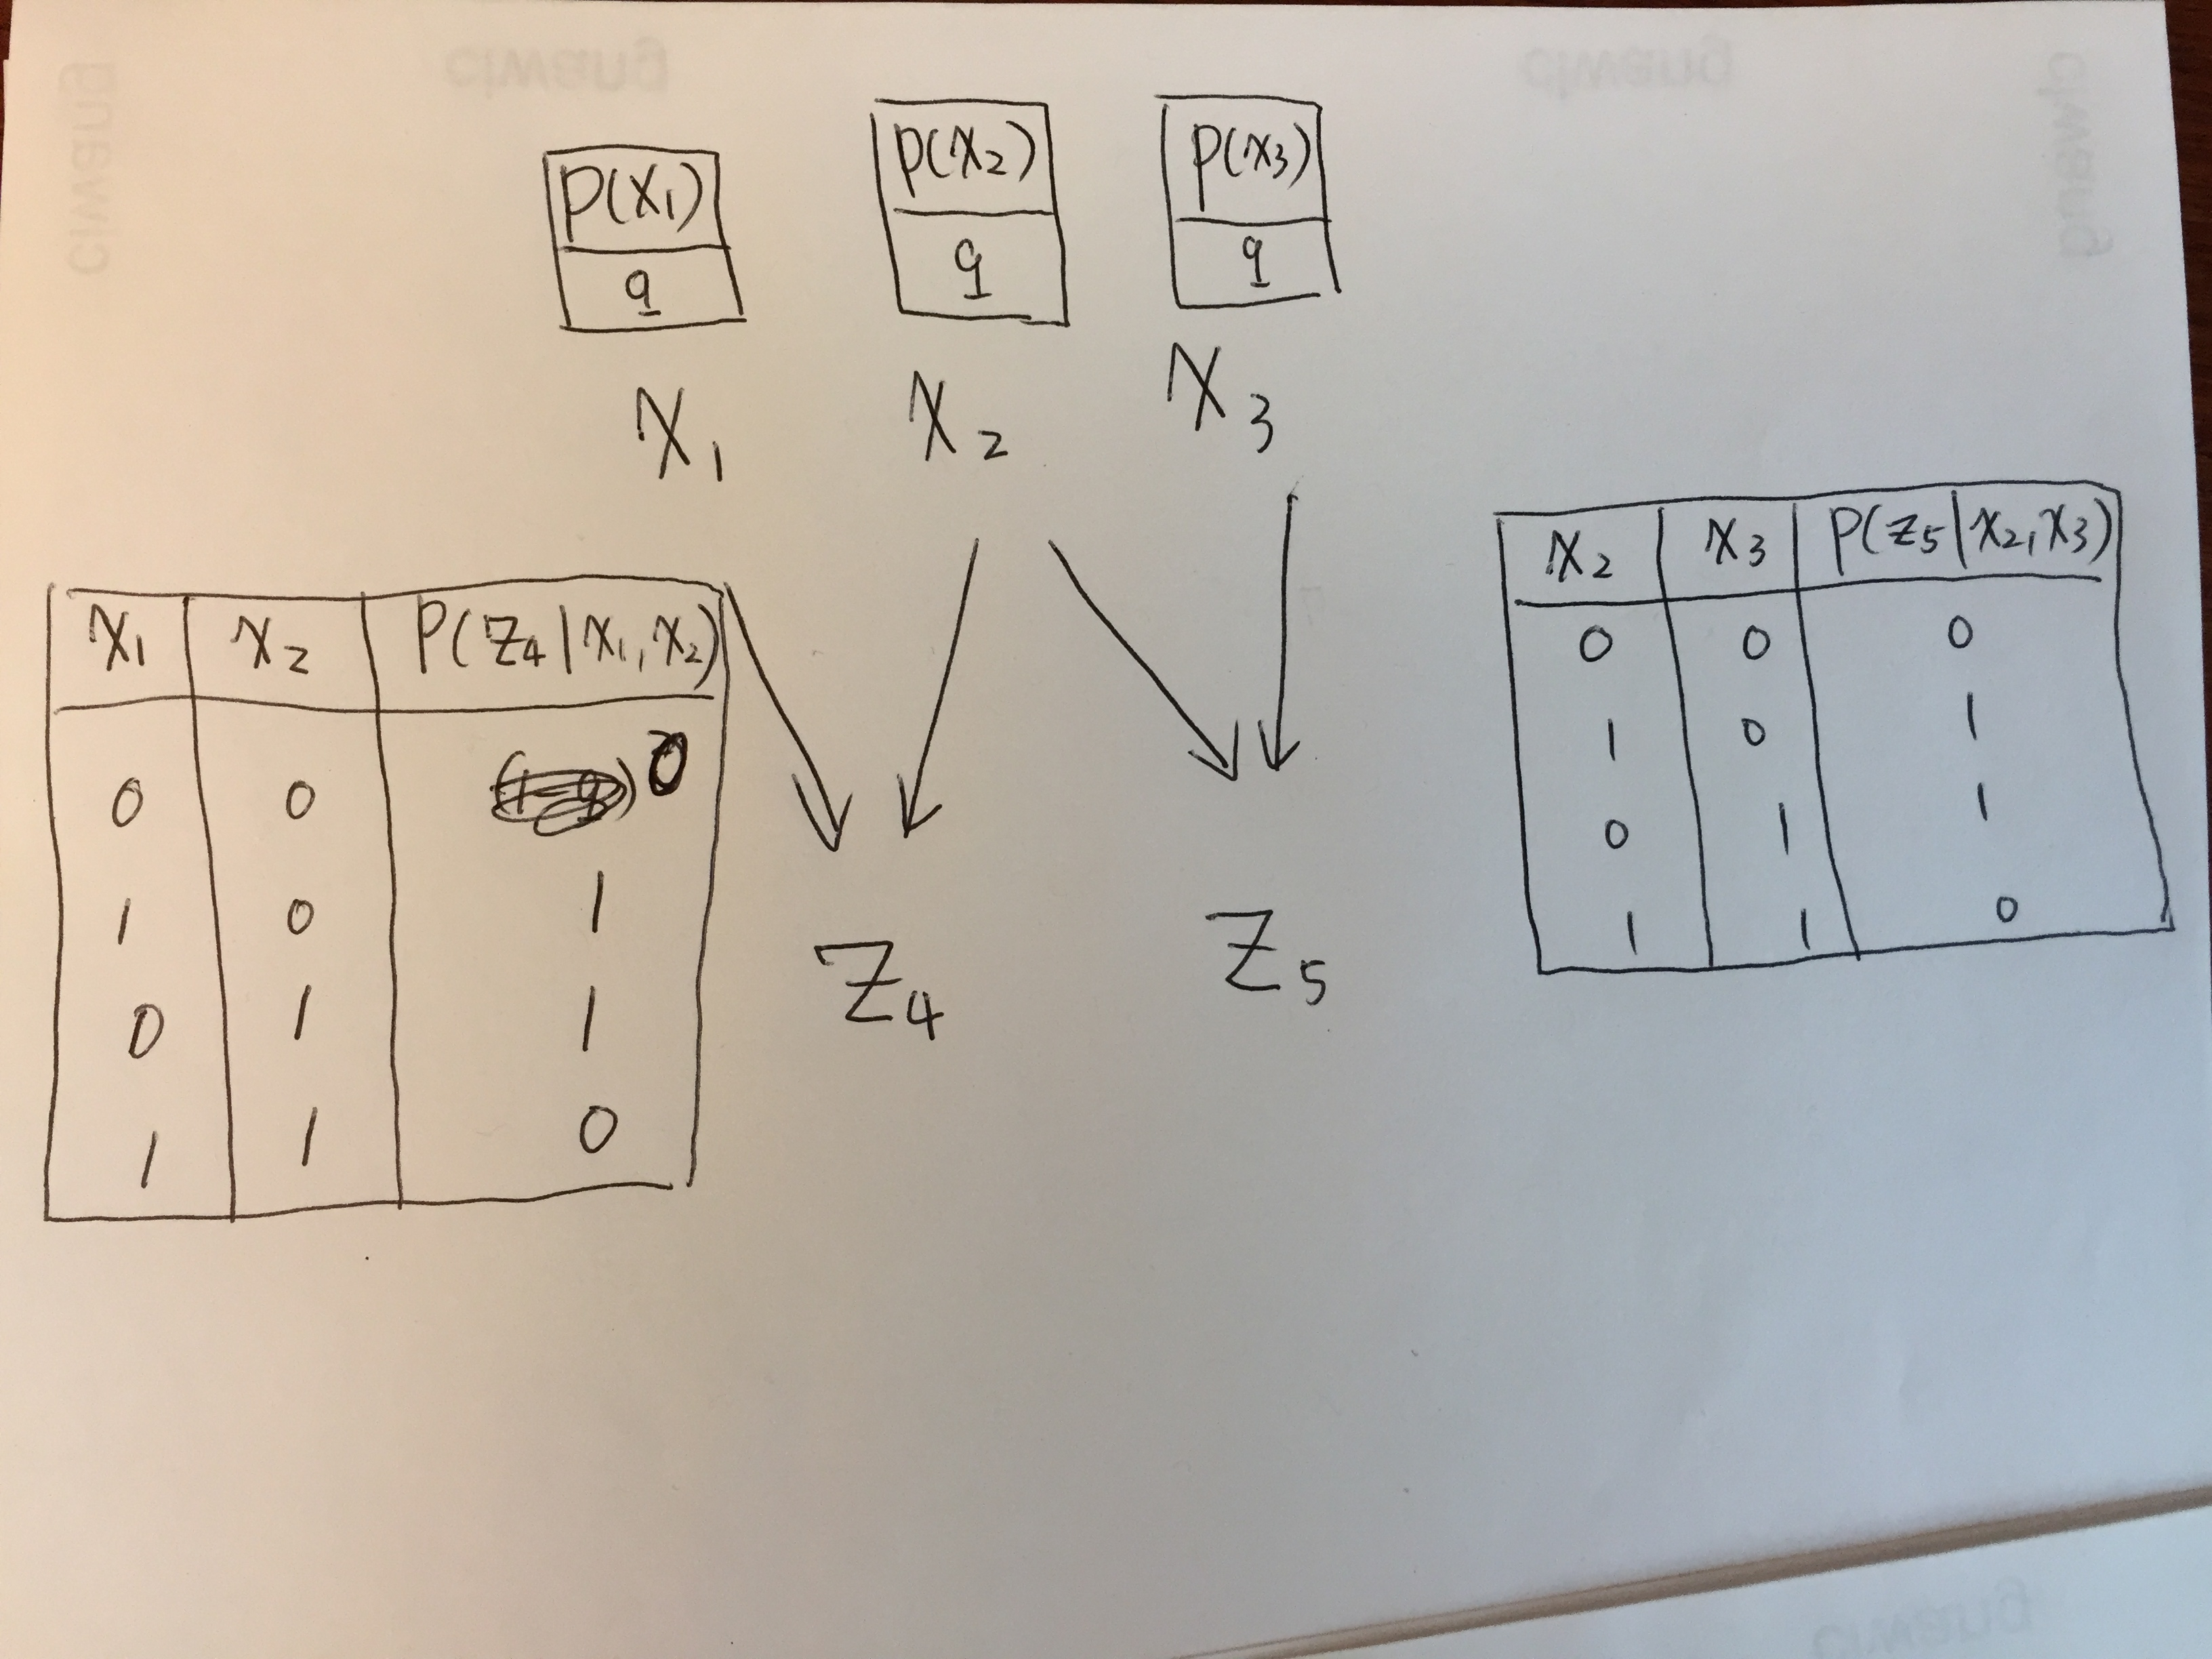
\includegraphics[width=0.5\columnwidth]{directed.jpg}

Independence relations: 

\begin{itemize}
\item $X_1, X_2$ are independent if $Z_4$ is unknown.
\item $X_2, X_3$ are independent if $Z_5$ is unknown.
\item $X_1, X_3$ are independent if (1) $X_2$ is known, or (2) $Z_4$ is unknown, or (3) $Z_5$ is unknown.
\item $Z_4, Z_5$ are independent if $X_2$ is known.
\item $Z_4, X_3$ are independent if (1) $X_2$ is known or (2) $Z_5$ is unknown.
\item $Z_5, X_1$ are independent if (1) $Z_4$ is unknown or (2) $X_2$ is known.
\end{itemize}

\item The undirected graph representation of the relation is shown below.

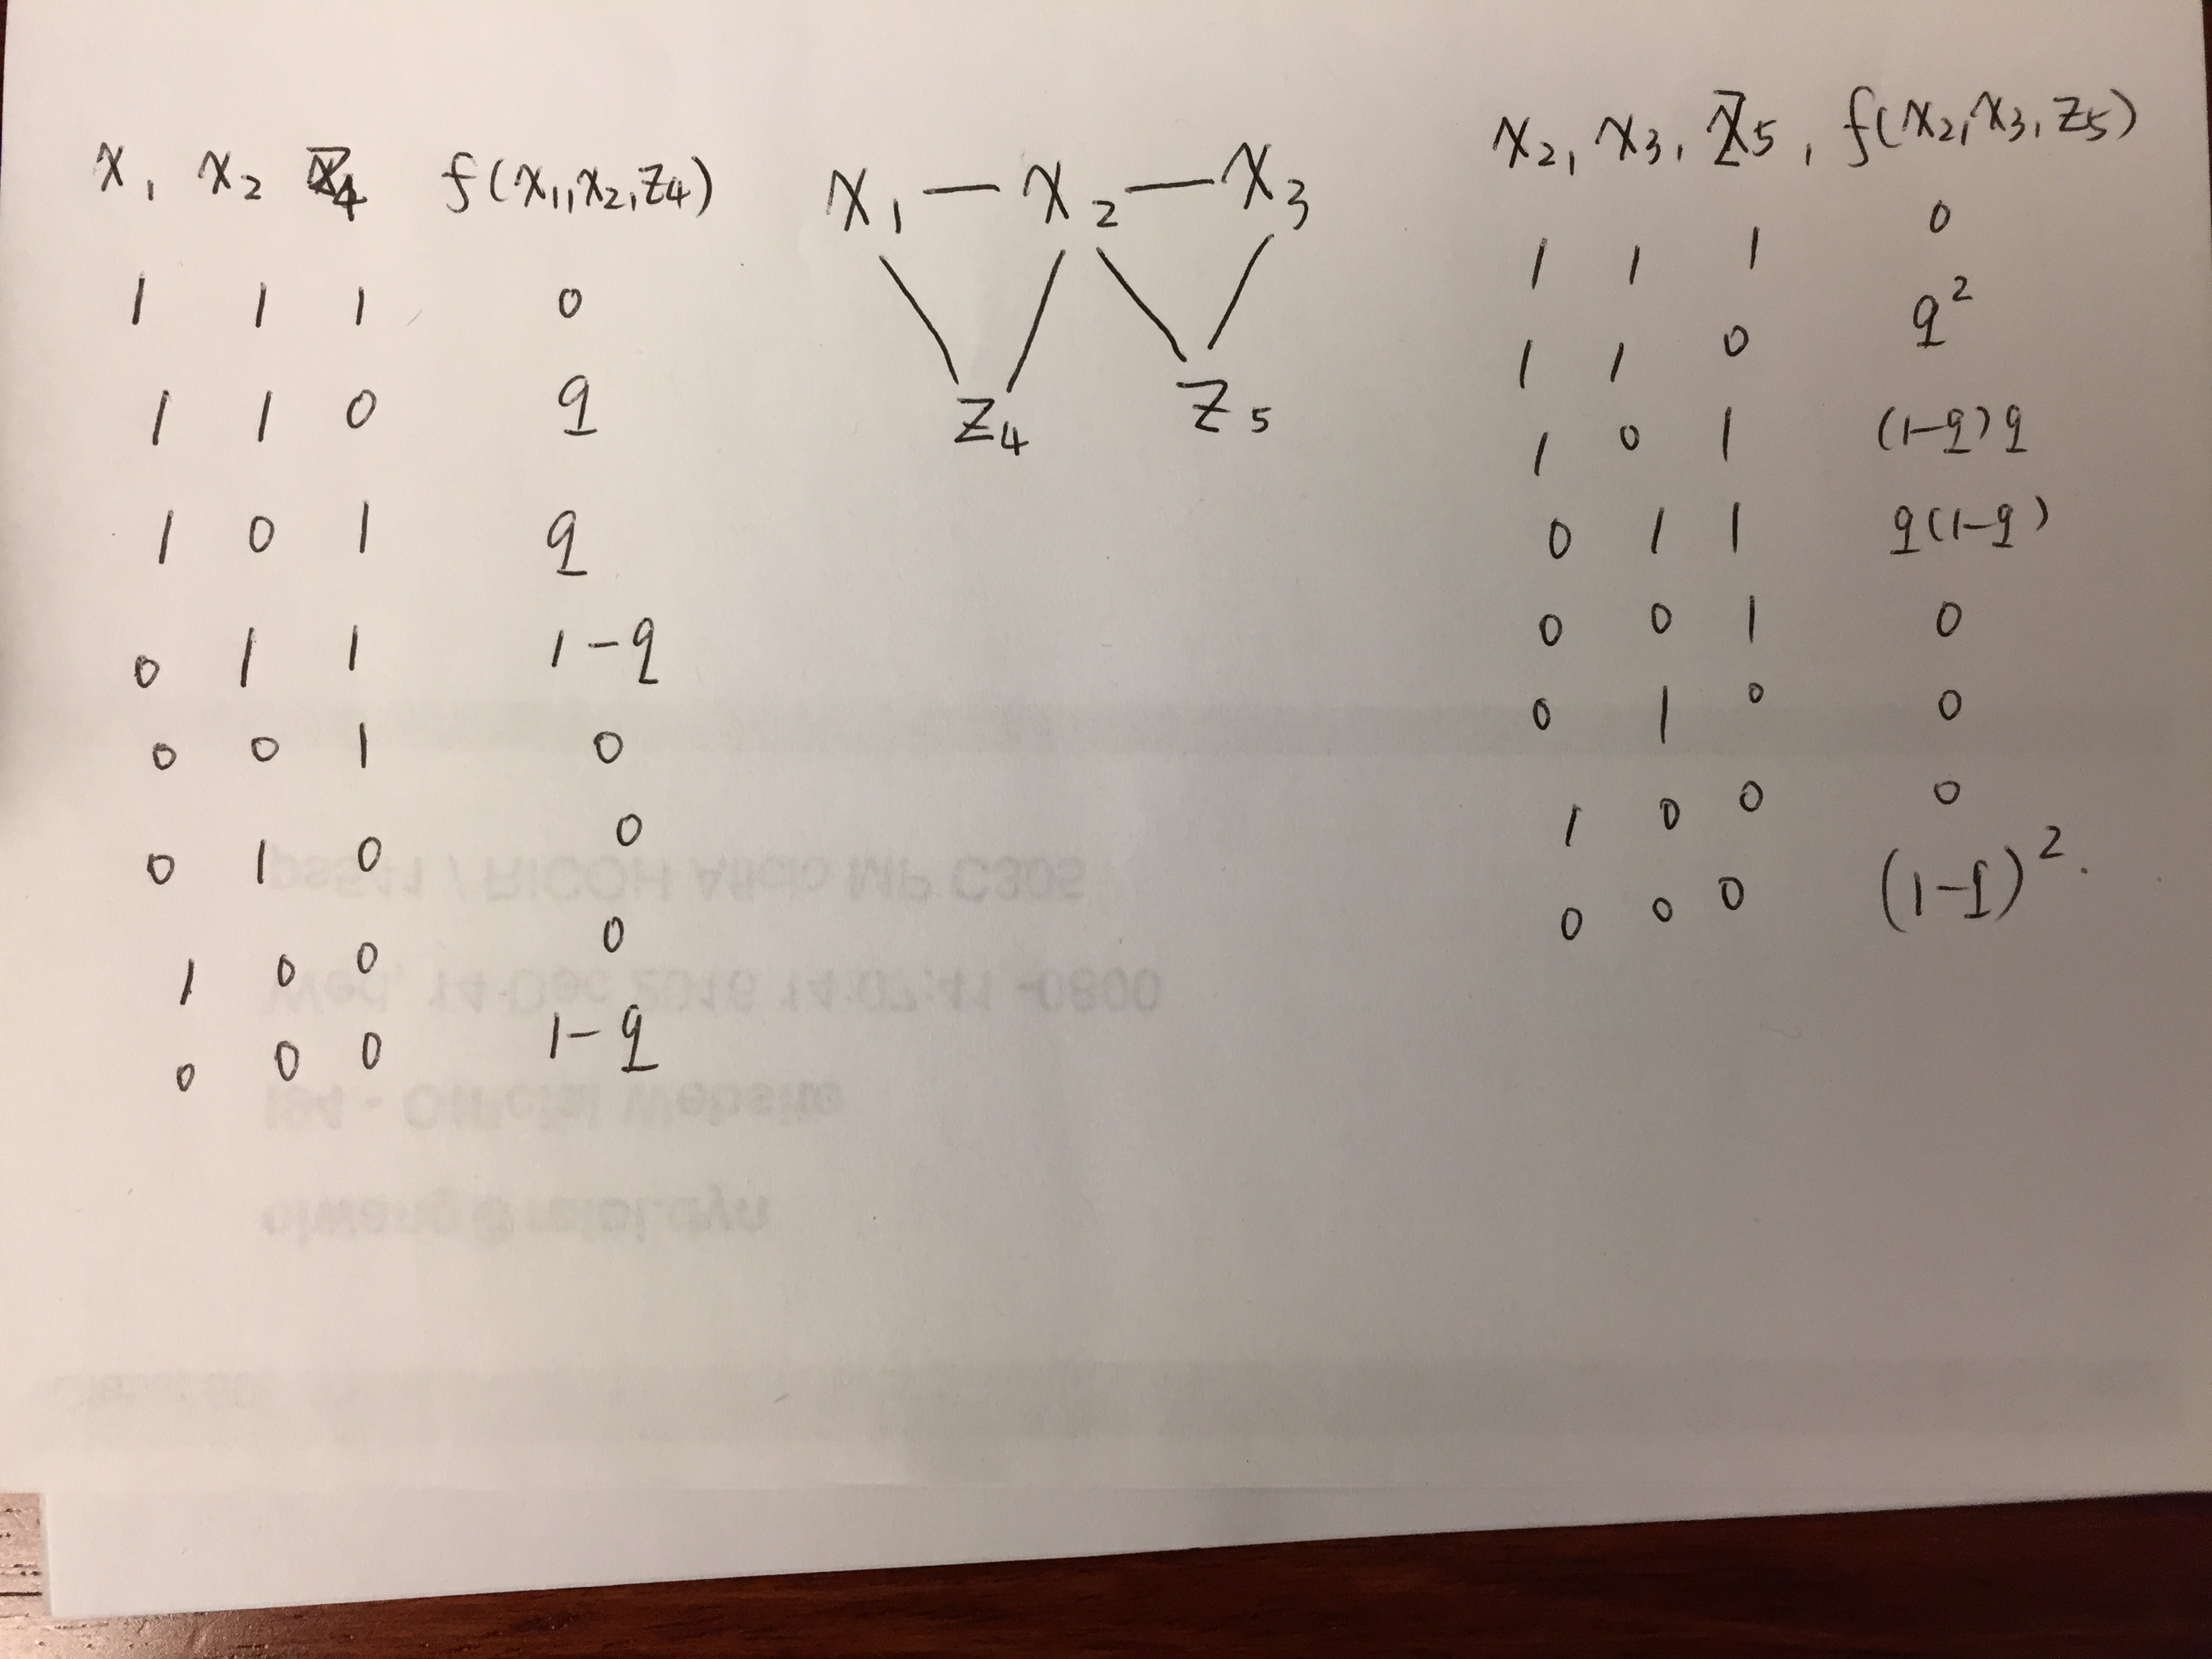
\includegraphics[width=0.5\columnwidth]{undirected.jpg}

\item If we want $Z_5\perp X_3$, we need $P(Z_5|X_3)=P(Z_5)$, i.e., $0.5 = 2q(1-q)$, which requires $q=0.5$.
Similarly, when $q=0.5$, $Z_4\perp X_1$. This information does not show up in either diagram.

\end{enumerate}

\section{BN2O Networks}

\begin{enumerate}
\item 
Given $F_i$ and the subset of parents $D_1,...,D_l$, their joint distribution is shown as follows:
\begin{align*}
P(F_i=f_i^0, D_1,...,D_l) 
=& \sum_{D_{l+1},...,D_k}P(F_i=f_i^0, D_1,...,D_l, D_{l+1}, ..., D_k)\\
=& \sum_{D_{l+1},...,D_k}P(F_i=f_i^0 | D_1,...,D_k)P(D_1,...,D_k)\\
=& \sum_{D_{l+1},...,D_k}\left[(1-\lambda_{i,0})\prod_{j=1}^{k}(1-\lambda_{i,j})^{d_{j}}\prod_{t=1}^{k}P(D_t)\right]\\
=& (1-\lambda_{i,0})\prod_{j=1}^l(1-\lambda_{i,j})^{d_{j}}\sum_{D_{l+1},...,D_k}\prod_{t=l+1}^k(1-\lambda_{i,t})^{d_t}P(D_t)\\
\end{align*}

Let $A=\sum\limits_{D_{l+1},...,D_k}\prod\limits_{t=l+1}^k(1-\lambda_{i,t})^{d_t}P(D_t)$ and $\lambda'_{i,0}=1-A(1-\lambda_{i,0})$, we have the updated CPD as follows: 
\begin{align*}
P(F_i=f_i^0|D_1,...,D_l)
= &(1-\lambda'_{i,0})\prod_{j=1}^l (1-\lambda_{i,j})^{d_j}\\
= &(1-\lambda_{i,0})\sum\limits_{D_{l+1},...,D_k}\prod\limits_{t=l+1}^k(1-\lambda_{i,t})^{d_t}P(D_t)\prod_{j=1}^l (1-\lambda_{i,j})^{d_j}
\end{align*}

In this way, the joint distribution of $F_i,D_1,...,D_l$ is maintained.

\item The posterior probability can be different from the original one since some dependencies may be removed due to the deletion of some parents. For example, given a network with $D_1,D_2,D_3$ and $F_1,F_2$, if $D_1,D_2$ are parents of $F_1$ and $D_2,D_3$ are parents of $F_2$. If we remove the node $D_2$, $D_1,D_3$ (or $F_1, F_2$) become conditionally independence, which was not the case for the original one.

If no new conditional independence relations are introduced, the distribution remains exact.
\end{enumerate}
\end{document}